\chapter{Hardware Realization} \label{sec:hwreal}

\section{Using a Discovery Board}

It has been proposed earlier in the text that STM32 Nucleo and Discovery development boards might be used as the hardware platform for this project. Indeed, a Discovery board with STM32F072~\cite{disco-f072} was used as a development platform for the majority of the GEX firmware. This inexpensive board may be used to try the GEX firmware without having access to the custom hardware.

\subsection{Discovery F072 Configuration and Pin Mapping}

This Discovery board is fitted with four \glspl{LED} on \gls{GPIO} pins PC6 through PC9, in a compass arrangement. The ``north'' \gls{LED}, PC6, is used as the GEX status indicator. The ``User'' button, connected to PA0, is mapped as the GEX Lock button, controlling the settings storage.

We advise the reader, as a potential user of this discovery board, to review its schematic diagram and ensure the solder-jumpers are configured correctly:

\begin{itemize}
	\item Jumpers SB20 and SB23 must be closed to enable the User \gls{USB} connector
	
	\item Jumper SB17 must be open and SB19 closed to use the 8\,MHz clock signal provided by the on-board ST-Link programmer; the internal USB-synchronized 48\,MHz oscillator will be used if the clock signal is not provided (SB19 open).
	
	\item Jumpers SB27 through SB32 should be closed to connect the \gls{GPIO} pins normally dedicated to the touch sensing strip to the board's header. 
	
	\item Capacitors C26 through C28 are sampling capacitors for the \gls{TSC}. There are, unfortunately, no jumpers available to disconnect them, and they interfere in high-speed signals on the used pins (PA3, PA7, PB1). The only solution is to carefully remove them from the board if the \gls{TSC} is not needed.
\end{itemize} 

An accelerometer \gls{IC} L3GD20 is fitted on the board. The chip is attached to SPI2 on pins PB13 (\gls{SCK}), PB14 (\gls{MISO}) and PB15 (\gls{MOSI}), with \gls{NSS} on pin PC0, and PC1 and PC2 used for interrupt flags. This chip cannot be disconnected or disabled and it is difficult to remove; care must be taken to avoid its interference on the used pins.

\section{GEX Hub}

GEX Hub was the first custom \gls{PCB} designed for GEX. It uses the same microcontroller as the Discovery board, thus the firmware modifications needed to make it work with this new platform were minimal.

The Hub board provides access to all the \gls{GPIO} pins using three flat-cable connectors, one for each port; they also contain a ground and power supply connection to make the connection of external boards or a breadboard easier, needing just one cable. The use of flat cables, however, is not mandatory---those connectors are based on the standard 2.54\,mm pitch pin headers, allowing the user to connect to them using widely available ``jumper wires''.

This board was produced in two revisions. The original model ( \cref{fig:gexhub1}) proved fully functional, except for the two connectors on the left side, the boot jumper and a programming header, which had the wrong footprints and could not be populated; this mistake was fixed by soldering the jumper from the bottom of the \gls{PCB}, and the programming header was never needed thanks to the USB bootloader working without issues. 

The updated revision removes the two problematic footprints altogether; a reorganization in the \gls{GPIO} connectors allowed them to be moved together with the other pins. Revision 1 used a dedicated header for the Boot jumper that was meant to be closed during normal operation, and removed only to enter the bootloader. Revision 2 moved the boot pin into the connector, and such arrangement would not be practical; the solution was to invert the jumper's logic by changing the Boot pull-up to a pull-down. The bootloader is now activated by inserting a regular 2.54\,mm jumper into the connector\footnote{A restart is required in all cases for the boot jumper changes to have effect}, as can be seen in \cref{fig:gexhub2}.

\begin{figure}[h]
	\centering
	\begin{subfigure}{.5\textwidth}
		\centering
		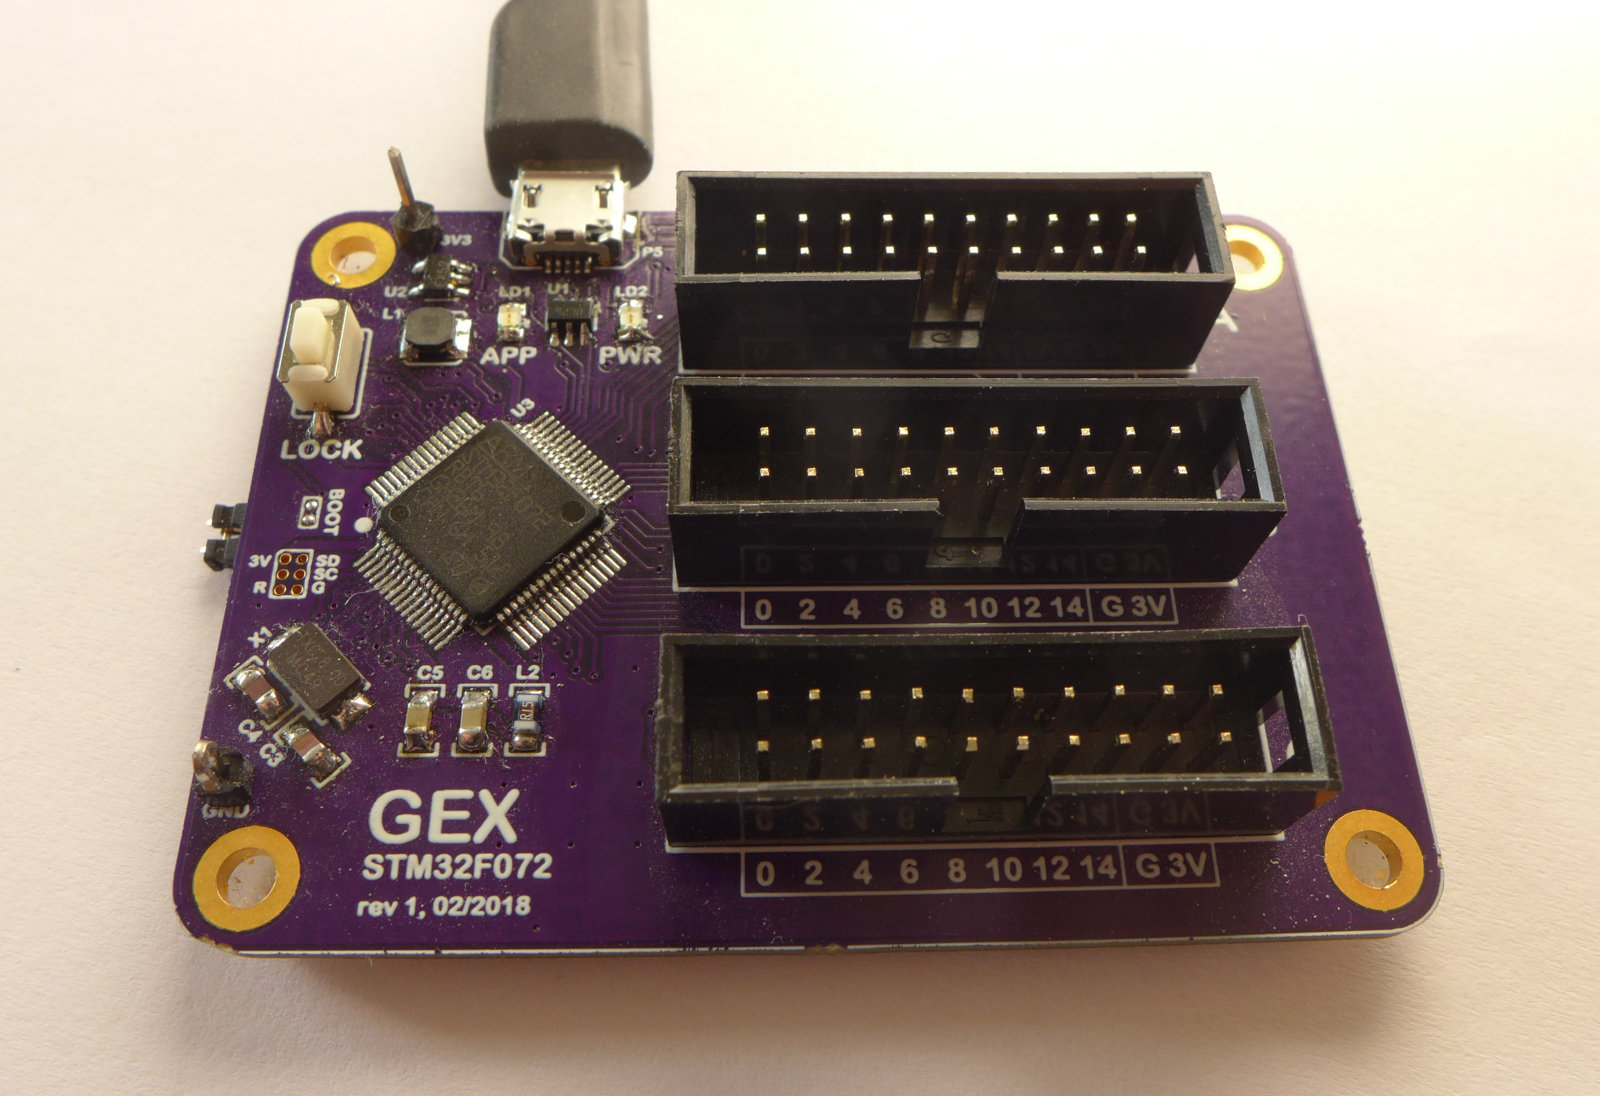
\includegraphics[width=.98\linewidth]{img/photo-hub1.jpg}
		\caption{\label{fig:gexhub1}Revision 1}
	\end{subfigure}%
	\begin{subfigure}{.5\textwidth}
		\centering
		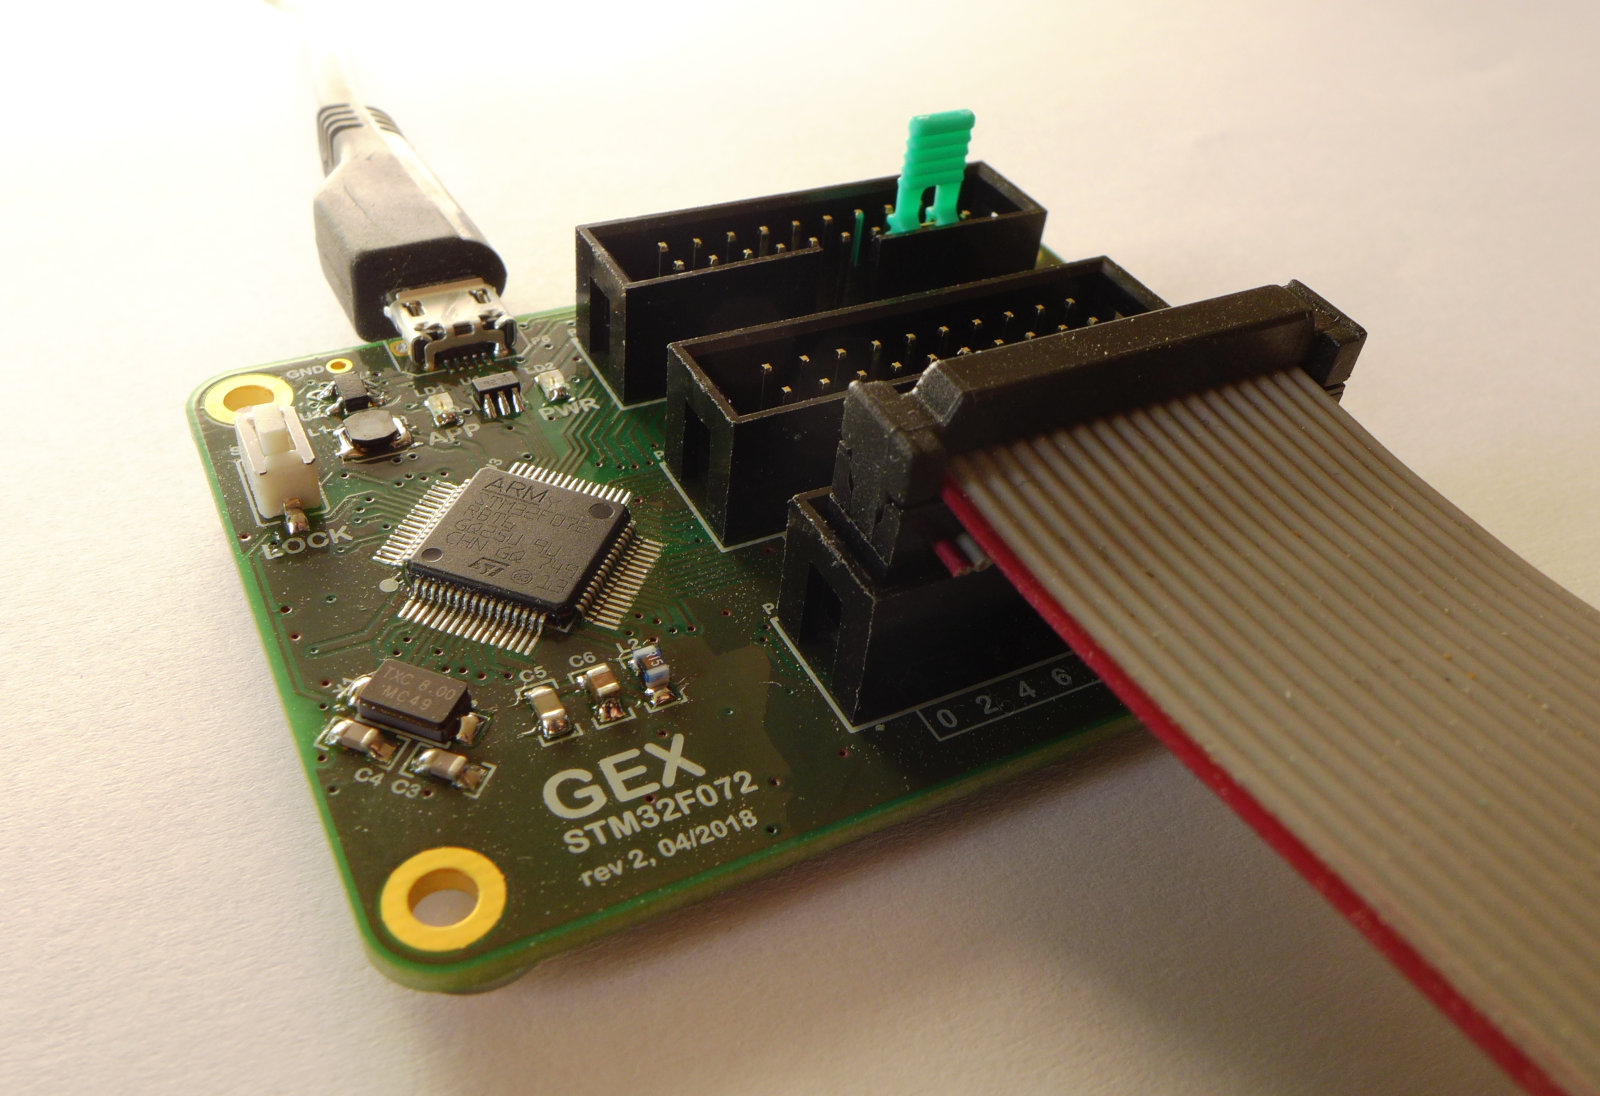
\includegraphics[width=.98\linewidth]{img/photo-hub2.jpg}
		\caption{\label{fig:gexhub2}Revision 2}
	\end{subfigure}
	\caption[The GEX Hub module]{\label{fig:gexhub} Two revisions of the GEX Hub module, rev. 2 shown with the boot jumper and a flat cable.}
\end{figure}


\section{GEX Zero}

Our desire to re-use the form factor of the Raspberry Pi Zero to exploit the existing market with add-on boards and cases for it has been revealed already in \cref{sec:formfactors}. This was brought to fruition with GEX Zero, the second realized prototype board (counting the two revisions of GEX Hub as one).

GEX Zero exactly copies the dimensions of the Pi Zero, which introduces several challenges:

\begin{itemize}
	\item It must be a one-sided board, with no components on the bottom; this is needed for acrylic cases which sit flatly against the \gls{PCB}, with a cut-out for the pin header.
	\item Buttons and the USB connector have to exactly align with connectors on the Pi Zero to fit the openings in its cases.
	\item The board size is fixed, and rather small; we used only two layers to save production cost, but this proved a significant challenge and the electrical characteristics of some connections may not be ideal.
	\item To make use of the Raspberry Pi add-on boards, called HATs or pHATs, a particular organization of the pin header is required. This is discussed in more detail below.
\end{itemize}

\subsection{Finding the Best Pin Assignment}

Like our STM32 microcontroller, the Broadcom processor on the Raspberry Pi multiplexes its \gls{GPIO} pins with alternate functions, and, likewise, each function is available only on a small selection of pins. A number of compromises had to be made to achieve maximum compatibility.

\todo[inline]{show the pi header mappings and the gex zero pin mappings}


\begin{figure}[h]
	\centering
	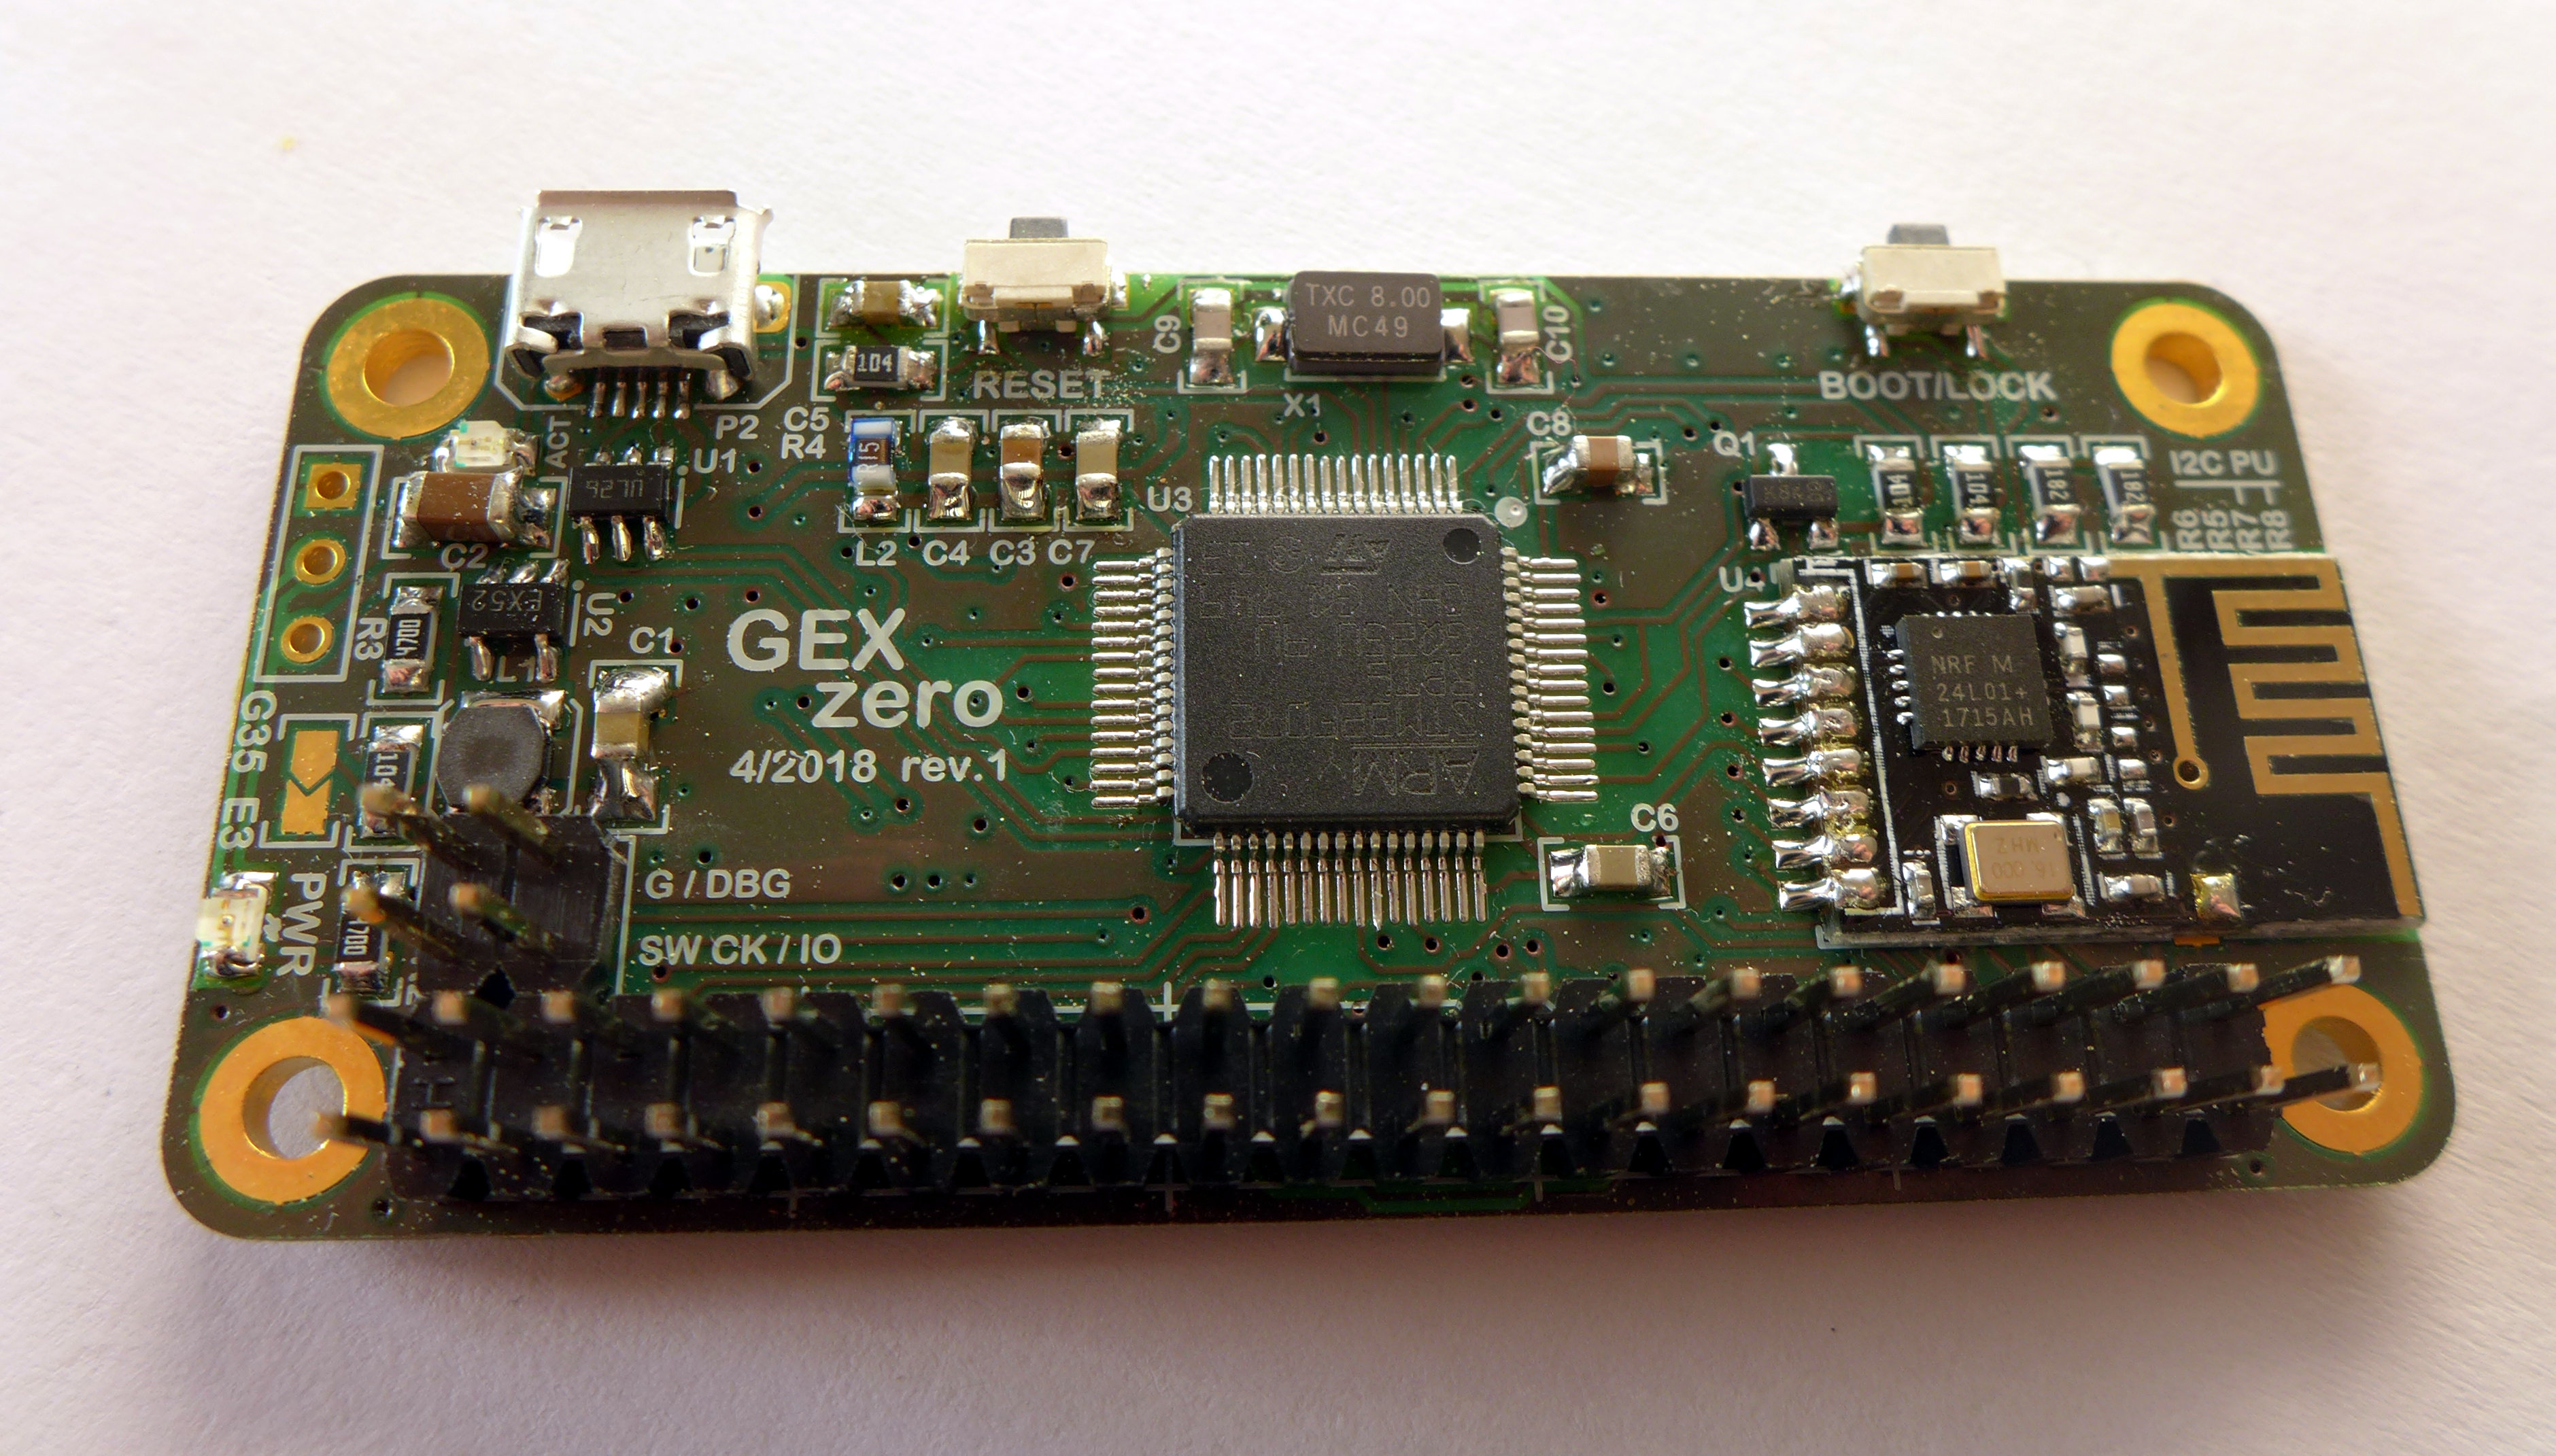
\includegraphics[width=.9\textwidth]{img/photo-zero-naked.jpg} \\
	\vspace{1mm}
	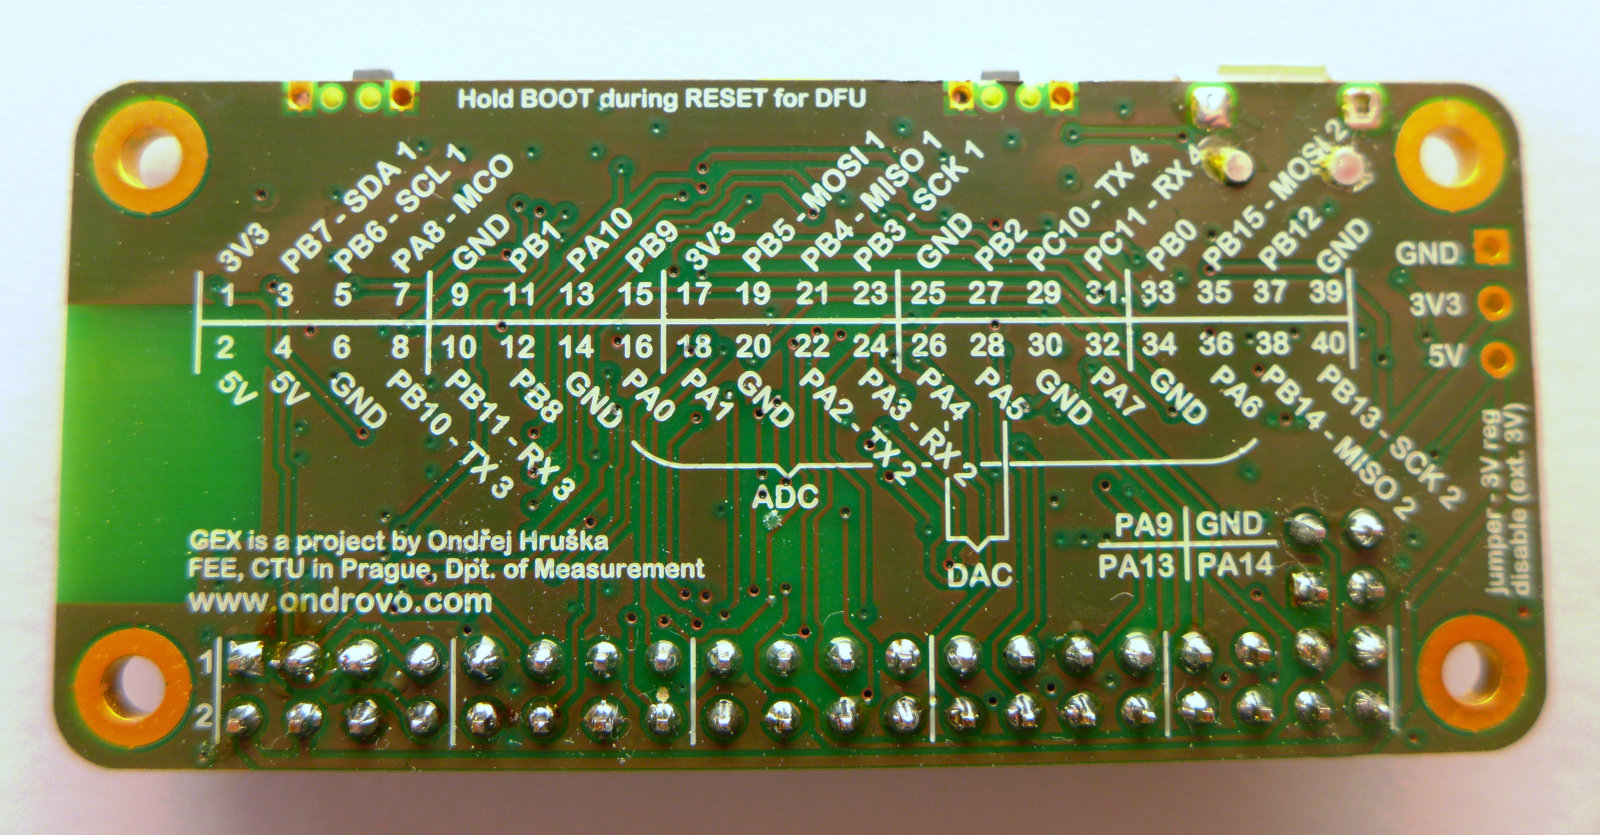
\includegraphics[width=.9\textwidth]{img/photo-zero-naked-bottom.jpg}
	\caption[The GEX Zero module]{\label{fig:gexz}GEX Zero, top and bottom side}
\end{figure}

\begin{figure}[h]
	\centering
	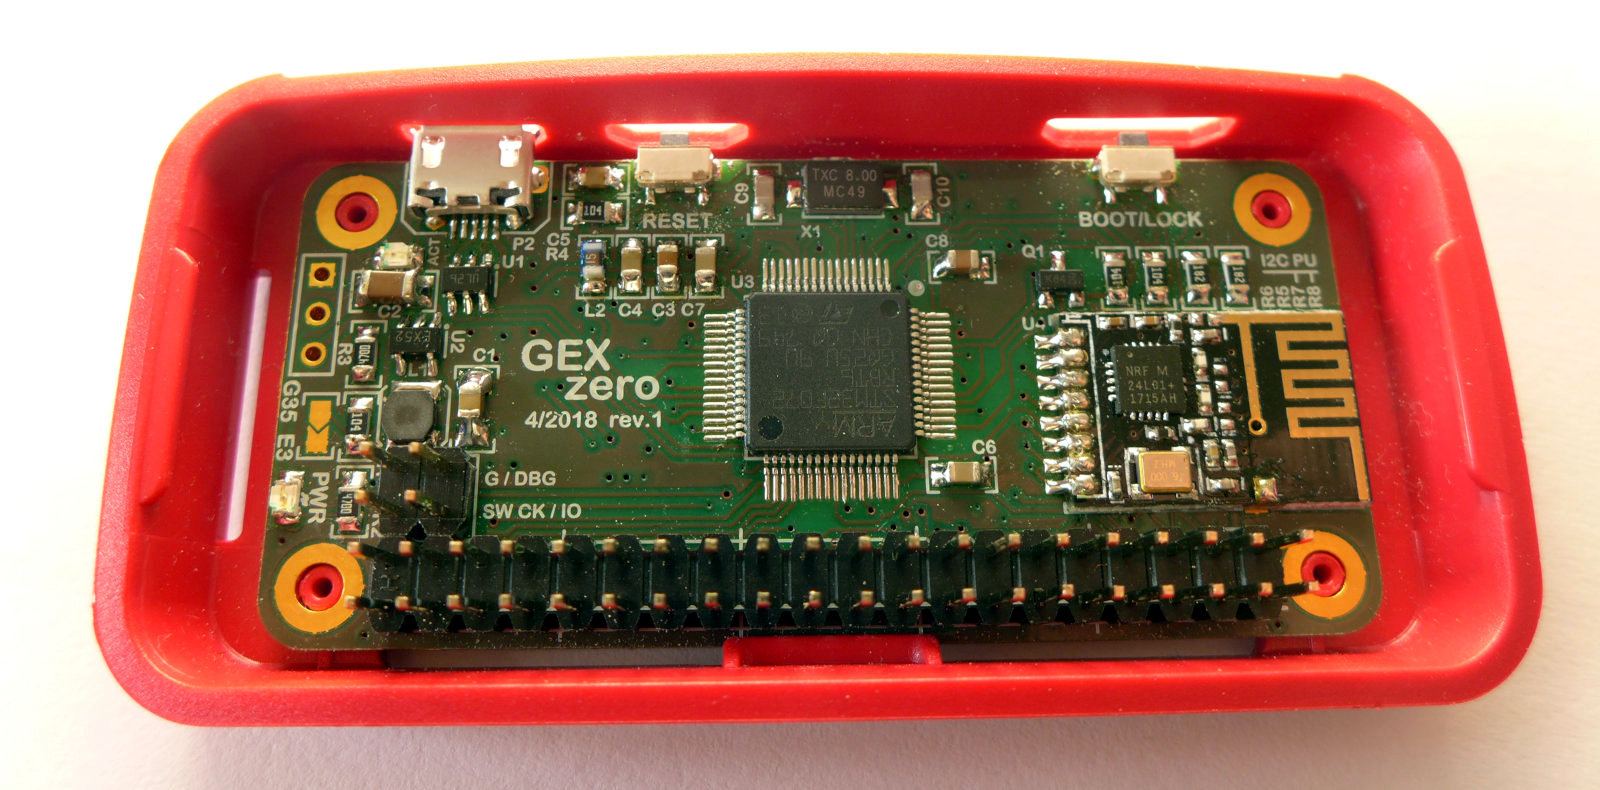
\includegraphics[width=.9\textwidth]{img/photo-zero-picase.jpg} \\
	\vspace{1mm}
	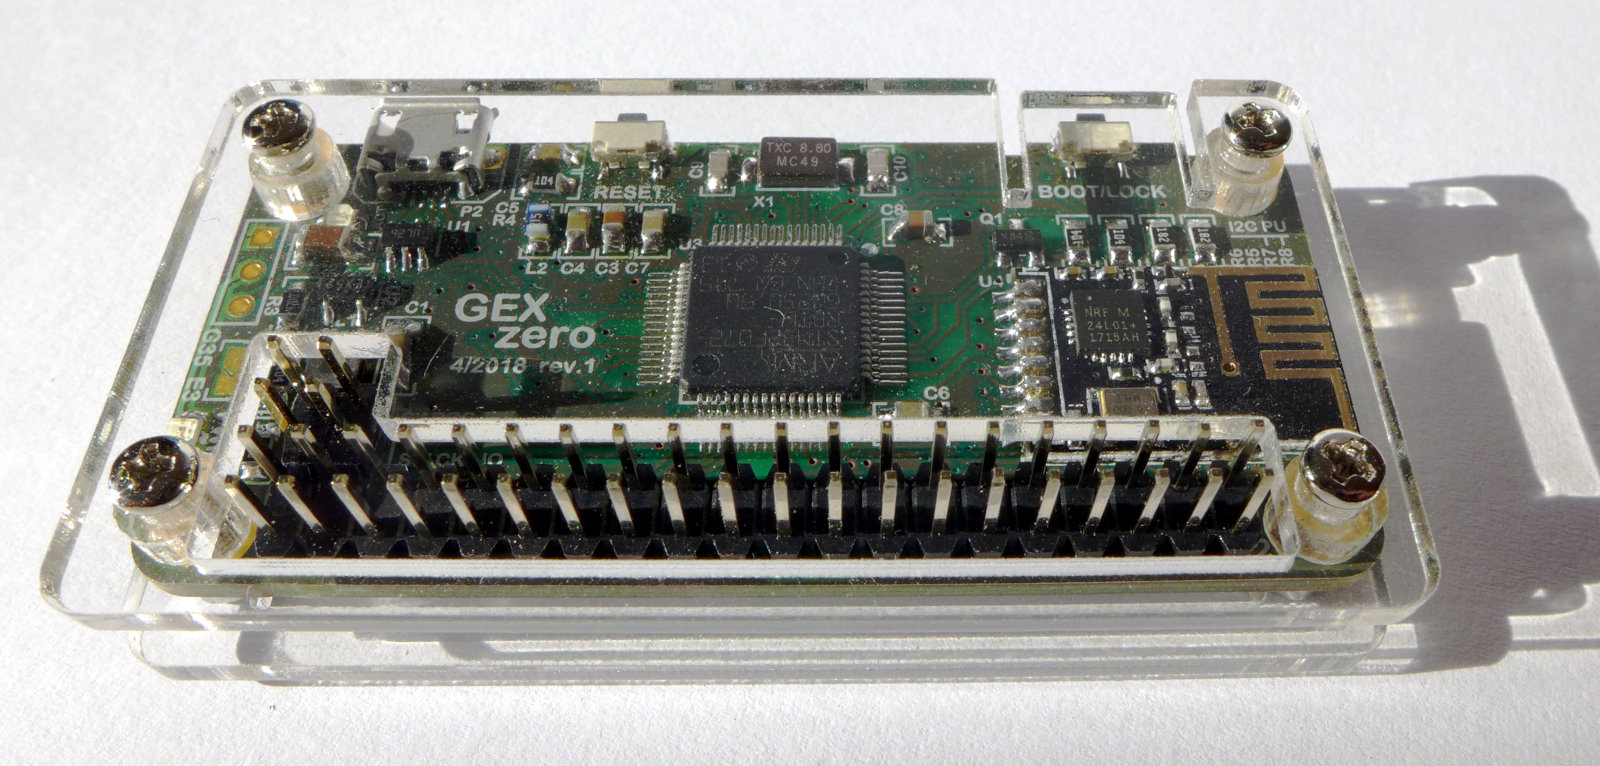
\includegraphics[width=.9\textwidth]{img/photo-zero-transparent.jpg}
	\caption[The GEX Zero module]{\label{fig:gexzcases}GEX Zero in the official Raspberry Pi Zero case and an aftermarket acrylic case}
\end{figure}


\section{Wireless Gateway}

\cref{fig:gwxgw}

\todo[inline]{TODO about the gateway ..}


\begin{figure}[h]
	\centering
	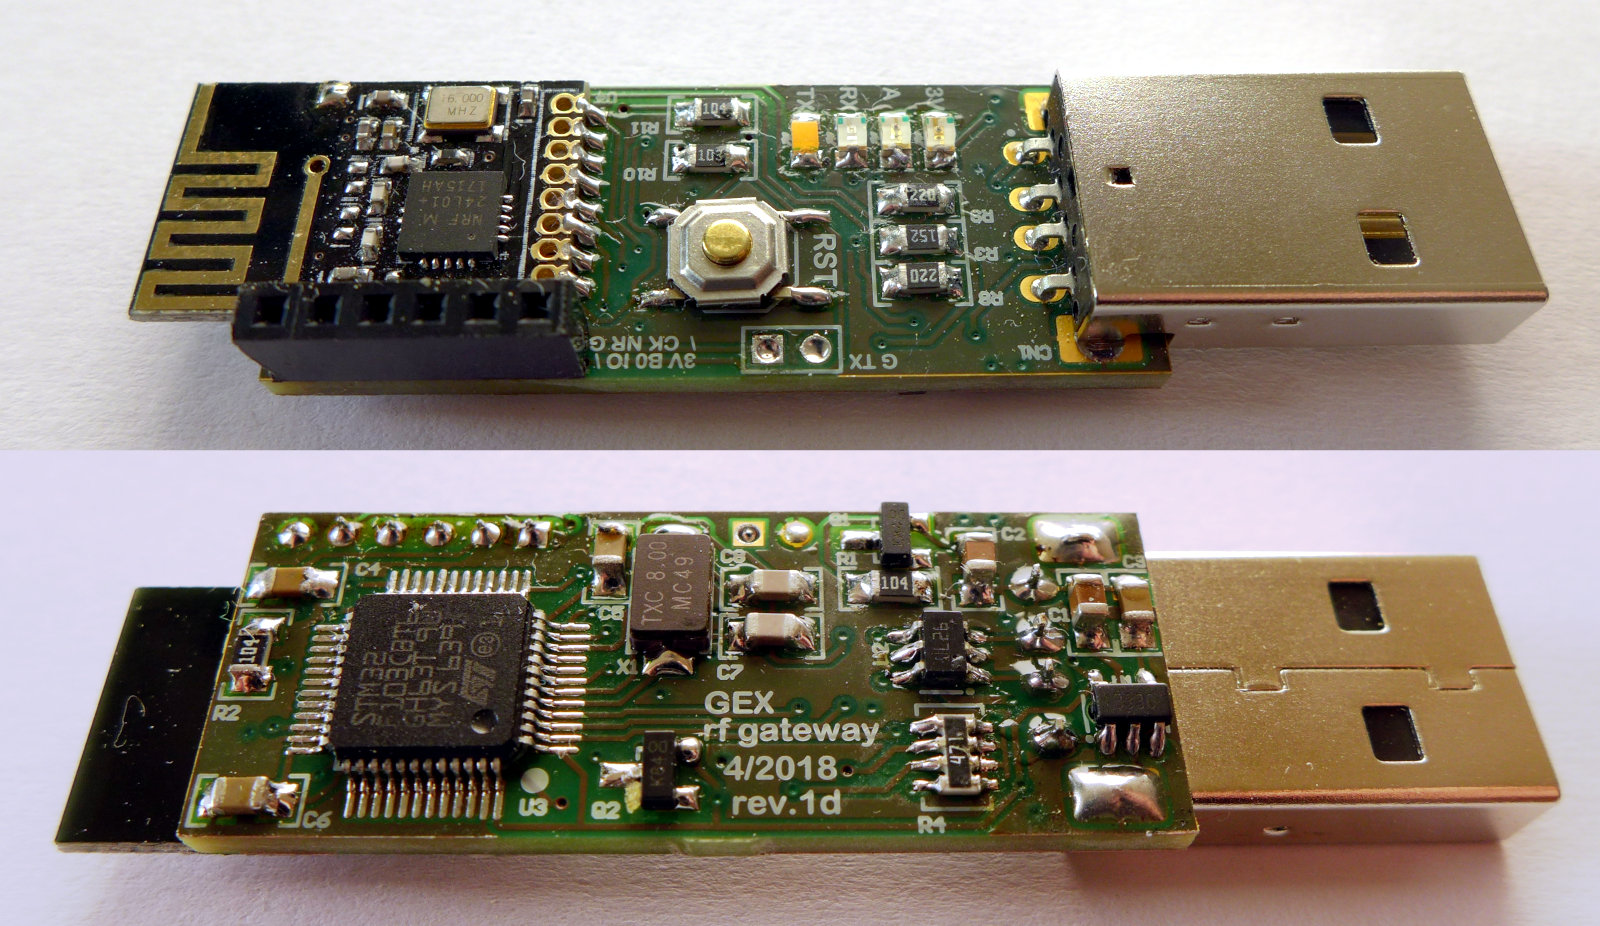
\includegraphics[width=.9\textwidth]{img/photo-rfdongle.jpg}
	\caption{\label{fig:gwxgw}The wireless gateway module (top and bottom side)}
\end{figure}


